\chapter{Γενετικοί Αλγόριθμοι}
\label{geneticAlgorithms}
Οι Γενετικοί Αλγόριθμοι (ΓΑ) είναι μέθοδοι εξερεύνησης, βελτιστοποίησης και μηχανικής μάθησης. Εμπνευσμένοι από τη Θεωρία της Εξέλιξης των Ειδών που θεμελίωσε ο Κ. Δαρβίνος, κάνουν χρήση της εξελικτικής διαδικασίας για την επίλυση υπολογιστικών προβλημάτων και την αναζήτηση ολικά βέλτιστων λύσεων, όπως ακριβώς και τα υπόλοιπα είδη αλγορίθμων του τομέα της Εξελικτικής Υπολογιστικής: ο Γενετικός Προγραμματισμός και οι Εξελικτικοί Αλγόριθμοι.

\section{Βιολογία και Γενετικοί Αλγορίθμοι}
Οι πρώτες εξελικτικές θεωρίες αναδύθηκαν στις αρχές του 19ου αιώνα, υποστηρίζοντας ότι τα είδη του φυσικού κόσμου συμμετέχουν και έχουν προκύψει από μία διαδικασία συνεχούς και αέναης εξέλιξης. Βασιζόμενοι στο έργο του Jean Batista Lamark που απέρριπτε την ιδέα ότι οι μορφές ζωής είναι αμετάβλητες, οι Darwin και Wallace, ανεξάρτητα ο ένας από τον άλλον, ανέπτυξαν την επαναστατική ιδέα της φυσικής επιλογής, όπως αυτή εκφράζεται στο βιβλίο του πρώτου “\emph{The origin of species}".
 
Η εξελικτική θεωρία υποστηρίζει την ύπαρξη ενός \emph{γενοτύπου} στον κάθε οργανισμό, δηλαδή μίας σαφώς ορισμένης κατάστασης ή διάταξης των τιμών του γονιδιώματος στο εσωτερικό του κάθε οργανισμού. Υπενθυμίζουμε πως γονιδίωμα ονομάζουμε το σύνολο των χρωμοσωμάτων ενός οργανισμού σε ένα κύτταρο του. Η μετάφραση του γενοτύπου σε επίπεδο φυσικού κόσμου, δηλαδή τα φυσικά χαρακτηριστικά γνωρίσματα, οι ικανότητες, οι αδυναμίες και τα προτερήματα ενός οργανισμού, συνιστούν το \emph{φαινότυπο} του. Στη Φύση, οι γενότυποι ενός είδους διαφέρουν σημαντικά ανάμεσα στα άτομα που το συνιστούν\footnote{Εγκυκλοπαιδικά, ο άνθρωπος διαφέρει σημαντικά από την πλειονότητα των άλλων ειδών στη Γη, καθώς κάθε άτομο διαφέρει λιγότερο από ένα οποιοδήποτε άλλο σε σχέση με άλλα είδη. Αυτό είναι το αποτέλεσμα μίας πληθυσμιακής συμφόρησης (bottleneck) στην Ιστορία εξέλιξης του ανθρώπινου είδους και οφείλεται στην υπερηφαιστιακή έκρηξη στη σημερινή λίμνη Toba στη Σουμάτρα Ινδονησίας, στα $73000\pm4000$ Π.Χ. Ο δεκαετής χειμώνας που προέκυψε από την κάλυψη του ουρανού από ηφαιστειακή τέφρα έφερε το ανθρώπινο είδος, που μέχρι εκείνη την περίοδο πιστεύεται ότι εδραζόταν στην Ανατολική Αφρική, στα πρόθυρα της ολοκληρωτικής εξάλειψης, μειώνοντας τον πληθυσμό του σε μερικές χιλιάδες άτομα (3.000 - 10.000). Η γονιδιακή δεξαμενή (genetic pool) συρρικνώθηκε σε τεράστιο βαθμό, στα άτομα που ήταν πλέον κατάλληλα για επιβίωση στις ακραίες εκείνες συνθήκες.}, ως αποτέλεσμα της εξελικτικής διαδικασίας, μέσω της οποίας τα άτομα τα οποία είναι καταλληλότερα για επιβίωση στο περιβάλλον τους, θα αναπαράγονται με μεγαλύτερη πιθανότητα\footnote{Τα άτομα που είναι καταλληλότερα για επιβίωση στο περιβάλλον τους, αναπαράγονται με μεγαλύτερη πιθανότητα καθώς, ενδογενώς, σκοπός του κάθε είδους είναι η διαιώνισή του. Κάθε άτομο θα επιλέξει ένα ταίρι του αντίθετου φύλλου για αναπαραγωγή, τέτοιο που να του εξασφαλίζει πρωτίστως την επιβίωση των απογόνων του και δευτερευόντως την ευημερία του.}, κληροδοτώντας στα παιδιά τους μέρος των γονιδίων τους και, έτσι, πολλαπλασιάζοντάς τα (survival of the fittest). Παράλληλα με τη διαδικασία \textit{διασταύρωσης} των γονιδίων ανάμεσα στους αρσενικούς και θηλυκούς προγόνους, εισάγονται, τυχαία, νέα χαρακτηριστικά στον πληθυσμό του είδους με το μηχανισμό της \textit{μετάλλαξης}.

Η παραπάνω περιγραφόμενη διαδικασία αποτελεί και το πλαίσιο λειτουργίας των Γενετικών Αλγορίθμων. Ένας Γενετικός Αλγόριθμος είναι μία συνεχής διαδικασία που μεταχειρίζεται έναν \emph{πληθυσμό ατόμων} και στα πλαίσια της οποίας τα άτομα:
\begin{enumerate}
\item\emph{αναπαράγονται}, μεταφέροντας το γενότυπό τους στους απογόνους τους,
\item\emph{μεταλλάσσονται}, με καθαρά τυχαίο τρόπο,
\item\emph{ανταγωνίζονται}, καθώς ζουν σε περιβάλλοντα με περιορισμένους πόρους, και 
\item\emph{επιλέγονται} (για αναπαραγωγή) ως αναπόφευκτο αποτέλεσμα του ανταγωνισμού τους για τους παραπάνω πόρους.
\end{enumerate}

Τα άτομα του πληθυσμού σε έναν ΓΑ αναπαριστούν μία πιθανή λύση στο υποκείμενο πρόβλημα. Κάθε άτομο αποτελείται από μία διάταξη \textit{γονιδίων}, το καθένα από τα οποία εκφράζει και ένα χαρακτηριστικό του ατόμου. Η σύνθεση των γονιδίων σε μία ενότητα μέσα στο άτομο είναι το \textit{χρωμόσωμά} του. Για την ευκολότερη αναπαράσταση και επεξεργασία από τους υπολογιστές, τα γονίδια είναι κωδικοποιημένα δυαδικά, με σημασία ανάλογη προς το πρόβλημα προς επίλυση. Ωστόσο, οι γενικές αρχές των Γενετικών Αλγορίθμων είναι ανεξάρτητες από τον τρόπο αναπαράστασης των γονιδίων και του χρωμοσώματος, αλλά και του ίδιου το προβλήματος. Εδώ ακριβώς φανερώνεται και η αρετή των Γενετικών Αλγορίθμων στην επίλυση δυσνόητων (ή ακόμα και μη κατανοητών) προβλημάτων. Ο προγραμματιστής δεν χρειάζεται να γνωρίζει τις λεπτομέρειες των εσωτερικών χαρακτηριστικών του προβλήματος. Αρκεί να μπορεί να αναπαραστήσει τη δομή του \textit{χώρου αναζήτησης}\footnote{Ορίζουμε ως \emph{Χώρο Αναζήτησης} ενός προβλήματος το σύνολο όλων των δυνατών και έγκυρων λύσεων, μέσα στο οποίο ανήκουν και οι λύσεις του προβλήματος.} και να μπορεί να αξιολογήσει τα άτομα - λύσεις του προβλήματος.


Για την αξιολόγηση της ποιότητας κάθε ατόμου - λύσης, πάνω στην οποία βασίζεται η υλοποίηση της φυσικής επιλογής, χρησιμοποιείται μία συνάρτηση αξιολόγησης της ποιότητας, ή καταλληλότητας, κάθε ατόμου. Με άλλα λόγια, η \textit{καταλληλότητα} (fitness) είναι ένα μέτρο της ικανότητας του ατόμου για επίλυση του δεδομένου προβλήματος ή ενός μέρους αυτού. Καθώς η καταλληλότητα είναι η μοναδική μετρική με την οποία συγκρίνονται τα άτομα, η μέθοδος υπολογισμού της είναι κρίσιμης σημασίας. Η συνάρτηση αξιολόγησης, επομένως, θα πρέπει να διαχωρίζει με επιτυχία καλές από κακές λύσεις, αλλά και να δημιουργεί έμμεσα αποτελεσματική πίεση (fitness pressure) προς την αναπαραγωγή και επιβίωση των ατόμων που αποτελούν τις καταλληλότερες λύσεις για το πρόβλημα. 


Τέλος, αξίζει να παρατηρήσουμε τη στοχαστική φύση των εξελικτικής διαδικασίας. Πρώτον, όπως αναφέραμε, η μετάλλαξη είναι ένα καθαρά στοχαστικό γενετικό συμβάν, καθώς, στην πράξη, σφάλματα στη μεταφορά της γενετικής πληροφορίας είναι αναπόδραστα και απρόβλεπτα. Δεύτερον, και η ίδια η επιλογή δεν είναι αιτιοκρατική. Η ποιότητα, ή καταλληλότητα, του ατόμου είναι μεν η σημαντικότερη του παράμετρος, γιατί είναι μέτρο της ικανότητάς του για επιβίωση, υπάρχουν όμως πολλοί εξωτερικοί παράγοντες που μπορούν να μεταβάλλουν τη διαδικασία επιλογής. Μία ενδιαφέρουσα παράμετρος, που όμως ξεφεύγει από τα πλαίσια αυτής της εργασίας, είναι οι μετατοπίσεις του ορισμού της \emph{καταλληλότητας} από κάθε κοινωνία στο πέρασμα των αιώνων. Κάθε περίοδος επιτάσσει και τα δικά της κριτήρια για το τί συνιστά την καταλληλότητα, ανάλογα και με την ανθρώπινη πρόοδο και τις πτυχές της. Εβδομήντα χιλιάδες χρόνια πριν, κατάλληλος θεωρείτο αυτός που μπορούσε να αψηφίσει το εχθρικό περιβάλλον με τις φυσικές και πνευματικές του δυνάμεις και να υποτάξει τη φύση για το καλό της “αγέλης"\footnote{Παλαιότερα, και μέχρι την ανάπτυξη του εμπορίου μέσω μη χρηματιστικών συναλλαγών, απευθείας ανταλλαγών δηλαδή, ο άνθρωπος συγκροτούσε κοινωνίες μέχρι 150 άτομα.}. Στην Αρχαία Αθήνα η καταλληλότητα είχε διαφορετικό ορισμό. Το ίδιο και μετά από κάθε κοινωνικό, οικονομικό ή πολιτισμικό paradigm shift.


\section{Αλγόριθμος Εξέλιξης}
Μια γενική μορφή της διαδικασίας εξέλιξης για έναν απλό ΓΑ φαίνεται στον Αλγόριθμο \ref{alg:gaGeneralForm}.

\begin{algorithm}
\caption{Γενική Μορφή Γενετικού Αλγορίθμου.}
\label{alg:gaGeneralForm}
\begin{algorithmic}[1]
\STATE $\textbf{geneticAlgorithm}()$
\STATE $t \gets 0$
\STATE $P(t) \gets initializePopulation()$
\WHILE{$terminationConditionNotMet$}
  	\STATE $t \gets t+1$
  	\STATE $P(t) \gets Evaluate(P(t))$
	\STATE $P'(t) \gets SelectParentsFrom(P(t-1))$
	\STATE $P'(t) \gets Crossover(P'(t))$
	\STATE $P'(t) \gets Mutate(P'(t))$
	\STATE $P(t) \gets P'(t)$
\ENDWHILE
\end{algorithmic}
\end{algorithm}

Ο πληθυσμός των ατόμων ενός Γενετικού Αλγορίθμου εξελίσσεται μέσα από μία επαναληπτική διαδικασία \emph{επιλογής - διασταύρωσης - μετάλλαξης - αντικατάστασης} των ατόμων. 

Σε πρώτο στάδιο, ο πληθυσμός αρχικοποιείται, είτε τυχαία, είτε με βάση υπάρχουσα γνώση πάνω στο πρόβλημα που μεταφράζεται (στο πεδίο λύσεων) σε άτομα. Σε δεύτερο στάδιο, στην αρχή κάθε επανάληψης, αποτιμάται η καταλληλότητα των ατόμων του πληθυσμού, μέσω της συνάρτησης αξιολόγησης. Στη συνέχεια, ακολουθεί η εφαρμογή των τελεστών διασταύρωσης και μετάλλαξης, με αποτέλεσμα έναν πληθυσμό απογόνων που αντικαθιστά τον τρέχοντα πληθυσμό πριν την επόμενη επανάληψη.

Αναλύουμε παρακάτω τις διαφορετικές μεθόδους που μπορούν να ακολουθηθούν σε σχέση με τη φυσική επιλογή, και τους τελεστές διασταύρωσης και μετάλλαξης.

\section{Διαδικασία Φυσικής Επιλογής}
\label{sec:naturalSelectionProcess}
Η διαδικασία της Φυσικής Επιλογής προσομοιώνει το φυσικό μηχανισμό της επιβίωσης του ικανοτέρου: είναι ο μηχανισμός που καθορίζει τον τρόπο με τον οποίο επιλέγονται τα καταλληλότερα άτομα του πληθυσμού για αναπαραγωγή, ώστε να αποτελέσουν τη γενετική βάση του πληθυσμού της επόμενης γενιάς. 

Για τη δημιουργία του νέου πληθυσμού υπάρχουν δύο βασικές μέθοδοι \cite{buckland2002ai}:

\begin{enumerate}
\item \textbf{Ελιτισμός (Elitism)} είναι η διαδικασία κατά την οποία ένα κομμάτι του πληθυσμού, η επονομαζόμενη ελίτ, θα διοχετευθεί αυτούσιο στο νέο πληθυσμό, λόγω των καλών χαρακτηριστικών των ατόμων της, ενώ το υπόλοιπο κομμάτι του νέου πληθυσμού θα προκύψει μέσα από αναπαραγωγή των κατάλληλων γονέων του προηγούμενου πληθυσμού.
\item \textbf{Επιλογή Σταθερής Κατάστασης (Steady-State Selection)} είναι μία διαδικασία αντίθετη προς τον ελιτισμό. Το μεγαλύτερο κομμάτι του πληθυσμού μεταφέρεται αυτούσιο στο νέο πληθυσμό, ενώ κάποια άτομα (σχετικά λίγα), με χαρακτηριστικά χαμηλότερη καταλληλότητα, ή που πληρούν άλλα κριτήρια, αντικαθίστανται από νέα άτομα, προκύπτοντα από την αναπαραγωγή κατάλληλων γονέων.
\end{enumerate}

Η επιλογή των ατόμων του πληθυσμού που θα αποτελέσουν τους γονείς, μέσω της αναπαραγωγής των οποίων θα προκύψουν τα άτομα - απόγονοι, μπορεί να συντελεστεί με μία πληθώρα τρόπων. Όλοι όμως οι τρόποι αυτοί βασίζονται στη γενική ιδέα της πόλωσης της διαδικασίας επιλογής προς άτομα με μεγαλύτερη καταλληλότητα. Μέθοδοι όπως η \emph{επιλογή ρουλέτας} ή η \emph{στοχαστική καθολική επιλογή} αναθέτουν σε κάθε άτομο του πληθυσμού μία πιθανότητα επιλογής ανάλογη προς την καταλληλότητά του. Άλλα σχήματα επιλογής, όπως η \emph{επιλογή τουρνουά} ακολουθούν μία αιτιοκρατική προσέγγιση, κατατάσσοντας σε φθίνουσα σειρά καταλληλότητας τα άτομα του πληθυσμού και επιλέγοντας αυτά που βρίσκονται στις υψηλότερες θέσεις. 

Καθώς αυτή η εργασία χρησιμοποιεί αποκλειστικά την επιλογή ρουλέτας, την εξετάζουμε πιο αναλυτικά στην επόμενη παράγραφο.

\subsection{Επιλογή Ρουλέτας}
\label{subsec:rouletteWheelSelection}
Η επιλογή ρουλέτας υλοποιείται ως μια εξομοίωση πραγματικής ρουλέτας. Κάθε άτομο του πληθυσμού τοποθετείται σε ένα χωρίο της ρουλέτας, του οποίου το μέγεθος είναι ανάλογο της καταλληλότητας του ατόμου. Όσο περισσότερο ικανό είναι ένα άτομο $i$, τόσο μεγαλύτερο χωρίο θα πληρώσει, άρα και τόσο μεγαλύτερη πιθανότητα θα έχει να επιλεγεί. Για πληθυσμό $n$ ατόμων, αυτή η πιθανότητα είναι ίση με 

\begin{equation}
\label{eq:rouletteWheelSelectionWithoutNumerosity}
P(i) = \frac{fitness(i)}{\sum\limits_{j=1}^n fitness(j)}
\end{equation}
\\



Στον Αλγόριθμο \ref{alg:rwsGeneralForm} παραθέτουμε τον αλγόριθμο επιλογής ρουλέτας σε μορφή ψευδοκώδικα, δεδομένου του πληθυσμού $[P]$.
\\

\begin{algorithm}
\caption{Επιλογής Γονέα μέσω Επιλογής Ρουλέτας.}
\label{alg:rwsGeneralForm}
\begin{algorithmic}[1]
\STATE $\textbf{rouletteWheelSelection}(P)$
\STATE $F \gets sumOfIndividualsFitnessIn(P)$
\STATE $f \gets random[0,F]$
\STATE $s \gets 0$
\STATE $index \gets 0$
\WHILE{$s < f$}
	\STATE $index \gets index + 1$
	\STATE $f(i) \gets fitnessOfIndividualInSegment(i)$
	\STATE $s \gets s +f(i)$
\ENDWHILE
\STATE $parent \gets individualInSection(index)$
\end{algorithmic}
\end{algorithm}


\begin{figure}[htb]
 \begin{center}
    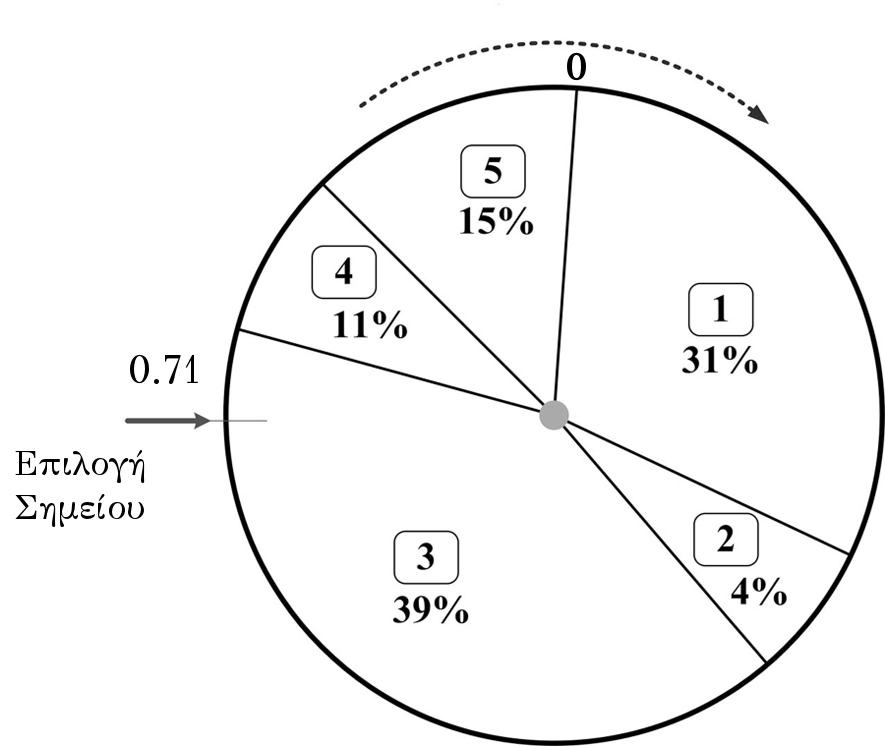
\includegraphics{./images/rouletteWheelSelection.png}
  \caption{Κατανομή ατόμων σε μία εικονική ρουλέτα.}
  \label{fig:rouletteWheelGA}
 \end{center}
\end{figure}





Στην αρχή υπολογίζεται το άθροισμα των καταλληλοτήτων $F$ των ατόμων που απαρτίζουν τον πληθυσμό, και στη συνέχεια, πολλαπλασιάζεται με έναν τυχαίο αριθμό στο διάστημα $[0,1]$, ώστε να προκύψει ένας τυχαίος αριθμός $f$ στο διάστημα $[0, F]$. Με αφετηρία το πρώτο άτομο, αθροίζουμε τις καταλληλότητες των ατόμων, σειριακά, έως ότου το άθροισμα ξεπεράσει τον αριθμό $f$. Το τρέχον άτομο θα αποτελέσει το ζητούμενο γονέα. Στο Σχήμα \ref{fig:rouletteWheelGA} παριστάνεται η παραπάνω διαδικασία για $f=0.71 \cdot F$.

Μία πιθανή διαφορά επίδοσης του μηχανισμού της επιλογής θα υπήρχε εάν το σημείο της αφετηρίας για την άθροιση των καταλληλοτήτων επιλεγόταν τυχαία κάθε φορά ή αν ο πληθυσμός ταξινομούταν πριν από κάθε γενετική επιλογή γονέα, με φθίνουσα σειρά καταλληλότητας των ατόμων του. Η διαφορά οφείλεται στη διάταξη των ατόμων στον πληθυσμό, καθώς, θεωρητικά, τα μέλη του πληθυσμού που βρίσκονται στο τέλος του, είναι αυτά που έχουν προστεθεί τελευταία και είναι, εν γένει, περισσότερο κατάλληλα, λόγω της πίεσης προς αυξανόμενη καταλληλότητα (fitness pressure). Αυτή η προσέγγιση είναι σημαντικά περισσότερο κοστοβόρα υπολογιστικά, αφού ο πληθυσμός αποτελείται από αριθμό ατόμων ανάλογο προς την πολυπλοκότητα του προβλήματος και τα σύνολα πραγματικών δεδομένων απαιτούν μερικές χιλιάδες έως δεκάδες χιλιάδες άτομα.

\section{Τελεστές Γενετικής Διασταύρωσης}
Η γενετική διασταύρωση στοχεύει στην ανάδειξη ατόμων που αποτελούν καλύτερες λύσεις του προβλήματος από τους προγόνους τους, με τον εντοπισμό αρκούντως κατάλληλων γονέων και την ανταλλαγή γενετικού υλικού (γονιδίων, όπως τα ορίσαμε παραπάνω) ανάμεσα στους δύο γονείς - χρωμοσώματα. Στις περισσότερες εφαρμογές ο αριθμός των απογόνων είναι δύο.

Κάποιες συχνά χρησιμοποιούμενες μέθοδοι διασταύρωσης παρουσιάζονται παρακάτω:

\begin{description}
\item\textbf{Διασταύρωση ενός σημείου}
\\
Επιλέγεται τυχαία ένα σημείο, κατά το μήκος των χρωμοσωμάτων. Αριστερά του σημείου διασταύρωσης, τα γονίδια του πρώτου απογόνου θα ταυτίζονται με αυτά του πρώτου γονέα, ενώ δεξιά του σημείου διασταύρωσης θα ταυτίζονται με τα γονίδια του δεύτερου. Για το δεύτερο απόγονο ισχύει το αντίθετο.
\item\textbf{Διασταύρωση δύο σημείων}
\\
Σε αυτή την περίπτωση επιλέγονται τυχαία δύο σημεία. Τα γονίδια δεξιά και αριστερά των σημείων διασταύρωσης μεταφέρονται αυτούσια από τους γονείς στους απογόνους, και αυτά μεταξύ των δύο σημείων εναλλάσσονται.
\item\textbf{Ομοιόμορφη Διασταύρωση}
\\
Χρησιμοποιεί τόσα σημεία διασταύρωσης όσα γονίδια διαθέτει το χρωμόσωμα. Κάθε γονίδιο ενός απογόνου αντιγράφεται από τον έναν γονέα ή τον άλλο, βάσει μιας δυαδικής μάσκας διασταύρωσης, η οποία δημιουργείται τυχαία για κάθε ζευγάρι γονέων, πριν ξεκινήσει η διαδικασία. Η μάσκα διασταύρωσης αποκτά την τιμή $1$ σε μία θέση σύμφωνα με μία δοσμένη πιθανότητα ομοιόμορφης διασταύρωσης.
\end{description}

Εμπειρικά, η πιθανότητα διασταύρωσης τοποθετείται στο διάστημα $[0.7, 0,9]$. Στην περίπτωση που δεν επιλεχθεί διασταύρωση, οι απόγονοι προκύπτουν ως αντίγραφα των γονέων. Στην Παρ. \ref{subsec:gmlaslcsCrossover} εξετάζουμε μία τέταρτη μέθοδο, ειδικά για τη διασταύρωση κανόνων πολυκατηγορικής ταξινόμησης.

\section{Τελεστές Γενετικής Μετάλλαξης}
Μετά τη διασταύρωση εφαρμόζεται η γενετική μετάλλαξη. Παρά την πληθώρα υλοποιήσεων τελεστών μετάλλαξης, όλοι λειτουργούν με τον ίδιο περίπου τρόπο. Σε αντίθεση με τη γενετική διασταύρωση, δέχονται ως είσοδο ένα μόνο χρωμόσωμα, ενώ εισάγουν νέες, τυχαίες τιμές στα γονίδια των απογόνων (τιμές που διαφορετικά μπορεί να μην είχαν εμφανιστεί), συμβάλλοντας σημαντικά στη γενετική ποικιλομορφία του πληθυσμού. Επιπρόσθετα, η έρευνα του χώρου αναζήτησης γίνεται πιο αποτελεσματική, καθώς, μειώνεται η πιθανότητα ο πληθυσμός να μείνει στάσιμος σε μία υπό-βέλτιστη λύση. Η πιθανότητα μετάλλαξης είναι σημαντικά μικρότερη από την πιθανότητα διασταύρωσης στους γενετικούς αλγορίθμους που χρησιμοποιούν δυαδική κωδικοποίηση και τοποθετείται στο διάστημα $[0.01, 0.1]$. 
\\
\\
Οι παραπάνω λειτουργίες της επιλογής, της διασταύρωσης και της μετάλλαξης, όταν εφαρμοστούν ξεχωριστά η καθεμία, έχουν αποδειχθεί αναποτελεσματικές \citep{goldberg02}. Όταν όμως συνδυαστούν, παράγουν χρήσιμα αποτελέσματα: ο συνδυασμός της επιλογής με τη διασταύρωση εισάγει μία λειτουργία καινοτομίας, ενώ ο συνδυασμός της μετάλλαξης με την επιλογή δημιουργεί γόνιμο έδαφος για συνεχή βελτίωση μέσω της τοπικής αναζήτησης.

\section{Γενετικοί Αλγόριθμοι και Εξόρυξη Δεδομένων}
Οι Γενετικοί Αλγόριθμοι έχουν τρεις βασικές εφαρμογές στην Εξόρυξη Δεδομένων \cite{freitas}:

\begin{enumerate}
\item\textbf{Εύρεση Κανόνων Ταξινόμησης}
\\
Η αναζήτηση και εξέλιξη κανόνων ταξινόμησης για τη δημιουργία προβλεπτικών μοντέλων μπορεί να υλοποιηθεί με τη χρήση Γενετικών Αλγορίθμων.
\item\textbf{Ομαδοποίηση}
\\
Η ομαδοποίηση αναφέρεται στη δημιουργία ομάδων από τα δεδομένα και χρησιμοποιείται σε εργασίες περιγραφής δεδομένων.
\item\textbf{Προεπεξεργασία Δεδομένων}
\\
Οι Γενετικοί Αλγόριθμοι μπορούν να χρησιμοποιηθούν για την επιλογή ή σύνθεση γνωρισμάτων ενός συνόλου δεδομένων.
\end{enumerate}

Καθώς η παρούσα εργασία χρησιμοποιεί τους Γενετικούς Αλγορίθμους αποκλειστικά για την εύρεση κανόνων ταξινόμησης, επεκτείνουμε την ανάλυση της εφαρμογής αυτής στην επόμενη ενότητα.

\subsection{Αναπαραστάσεις Κανόνων ως Χρωμοσώματα} 
\label{subsec:michiganPittsburg}
Για την αναπαράσταση των κανόνων σε μορφή χρωμοσώματος υπάρχουν δύο βασικές προσεγγίσεις.

\begin{enumerate}
\item\textbf{Αναπαράσταση Συνόλου Κανόνων ως Άτομο} (Pittsburg Approach)
\\
Ένα χρωμόσωμα αναπαριστά ένα σύνολο κανόνων, μη σταθερού μεγέθους, το οποίο αποτελεί και μία πλήρη λύση του προβλήματος. Με αυτή την προσέγγιση, λαμβάνονται υπόψη οι πιθανές αλληλεπιδράσεις των κανόνων, όμως δημιουργούνται χρωμοσώματα μεγάλου μεγέθους, καθιστώντας δυσχερή την κατασκευή αποτελεσματικών γενετικών τελεστών.
\item\textbf{Αναπαράσταση ενός Κανόνα ως Άτομο} (Michigan Approach)
\\
Κάθε κανόνας είναι και ένα χρωμόσωμα. Σε αντίθεση με την προσέγγιση Pittsburg, τα άτομα έχουν σταθερό μήκος, είναι μικρότερα σε μέγεθος και η κατασκευή των γενετικών τελεστών είναι σημαντικά ευκολότερη. Παρ' όλα αυτά, αυτή η μέθοδος αναπαράστασης δεν λαμβάνει ρητά υπόψη της τις πιθανές αλληλεπιδράσεις των κανόνων. Ο Γενετικός Αλγόριθμος, στην περίπτωση της προσέγγισης Michigan, προσπαθεί να κατασκευάσει ένα σύνολο κανόνων που “συνεργάζονται" ώστε όλοι μαζί να αποτελέσουν τη λύση του προβλήματος. Στην κατεύθυνση, λοιπόν, της διατήρησης της ποικιλότητας των κανόνων του πληθυσμού, χρησιμοποιούνται μέθοδοι όπως ο διαμοιρασμός καταλληλότητας, που τιμωρεί άτομα που ικανοποιούν μία ορισμένη συνθήκη ομοιότητας μεταξύ τους.
\end{enumerate}

Η παρούσα εργασία χρησιμοποιεί αποκλειστικά την προσέγγιση Michigan και, συνεπώς, στα επόμενα κεφάλαια θα προϋποθέτουμε αυτή τη γνώση.

\section{Περιορισμοί και Πλεονεκτήματα των Γενετικών Αλγορίθμων}
Σε γενικές γραμμές, οι Γενετικοί Αλγόριθμοι εμφανίζουν χαρακτηριστικά που δεν απαντώνται στους υπόλοιπους αλγορίθμους αναζήτησης και βελτιστοποίησης, ειδικά σε αυτούς που χρησιμοποιούν άπληστες ή αιτιοκρατικές προσεγγίσεις.

Οι Γενετικοί Αλγόριθμοι, αν και έχουν σαφέστατα μεγαλύτερο χρόνο εκτέλεσης από τις υπόλοιπες τεχνικές εξόρυξης δεδομένων, διαθέτουν λειτουργίες που μπορούν εύκολα να παραλληλοποιηθούν. Λόγω της μη αιτιοκρατικής τους φύσης, μπορούν να ανακαλύψουν λύσεις δύσκολα εντοπίσιμες, να ανακαλύψουν σχετικά εύκολα βέλτιστες λύσεις, αλλά και να αποφύγουν μη βέλτιστες λύσεις. Δυστυχώς, όμως, δυσκολεύονται, να βρουν το ακριβές σημείο της βέλτιστης λύσης χωρίς χρήση μεθόδων τοπικής έρευνας. Είναι εύρωστοι, καθώς λειτουργούν καλά παρουσία θορύβου στα δεδομένα, δεν είναι ευαίσθητοι σε (μικρές) αλλαγές των παραμέτρων τους, η λειτουργία τους δεν επηρεάζεται από ασυνέχειες του χώρου αναζήτησης και μπορούν να αποδώσουν το ίδιο καλά με άλλες τεχνικές σε προβλήματα ευρείας κλίμακας. Τέλος, μπορούν να εφαρμοσθούν για την επίλυση ποικίλων προβλημάτων αναζήτησης και βελτιστοποίησης, καθώς δεν απαιτούν την apriori κατανόηση της εσωτερικής δομής του προβλήματος-στόχου, και το μόνο που χρήζει αλλαγής είναι η αναπαράσταση των χρωμοσωμάτων και ο τρόπος αξιολόγησής τους. Υπάρχουν, βέβαια, και προβλήματα για τα οποία η κατασκευή μίας αποτελεσματικής αναπαράστασης χρωμοσωμάτων ή/και συνάρτησης αξιολόγησης είναι έργα από πολύπλοκα έως αδύνατα. Ο μεγάλος αριθμός των παραμέτρων τους και ο ακριβής χειρισμός τους, τέλος, είναι ένα δύσκολο καθήκον, ιδιαίτερα σε περιπτώσεις απουσίας εκ των προτέρων γνώσης του προβλήματος. 



